\subsubsection*{Training Insights}
Most ResNet101V2 trainings were not successful with only two trainings scoring a $\sigma < 0.18$. Apart from the models that massively over- or underestimated some galaxy masses, most models made smaller predictions resulting in a positive $\mu$. This behaviour was seen with most ResNet models. Especially for higher true masses, the difference between true and predicted mass was greater.


\subsubsection*{Best Performing Model}

\begin{figure}[H]
\centering
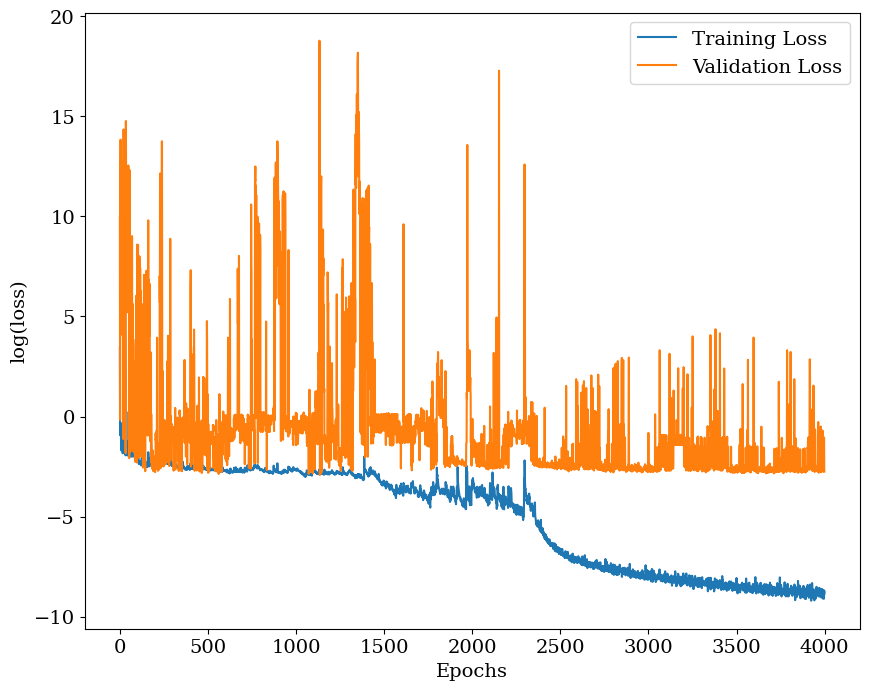
\includegraphics[width=.667\textwidth]{images/Chapter4/Res101V2/res101v2_history.png}
\caption{Training history of the best performing ResNet101V2 model.} 
\label{fig:resnet101v2_best_history}
\end{figure}

Despite the problems in training, the best performing ResNet101V2 model did quite well compared to the other models. With a $\sigma = 0.148$ it was the third best deep model of the ones I trained. Regardless of that, With a $\mu$ of $0.092$ it was the training that had the biggest difference between the predictions and the true masses of all trained models.


\begin{figure}[H]
\centering
\begin{subfigure}{.46\textwidth}
  \centering
  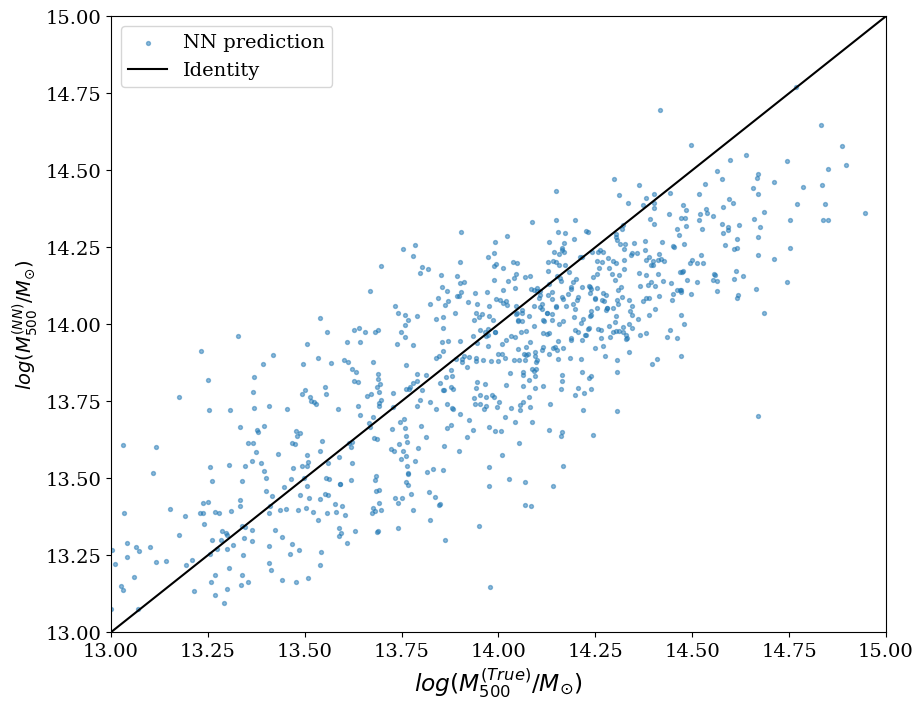
\includegraphics[width=\linewidth]{images/Chapter4/Res101V2/res101v2_test.png}
  \caption{Model predictions on the test set.}
  \label{fig:best_perf_resnet101v2_a}
\end{subfigure}%
\hspace{.6em}
\begin{subfigure}{.46\textwidth}
  \centering
  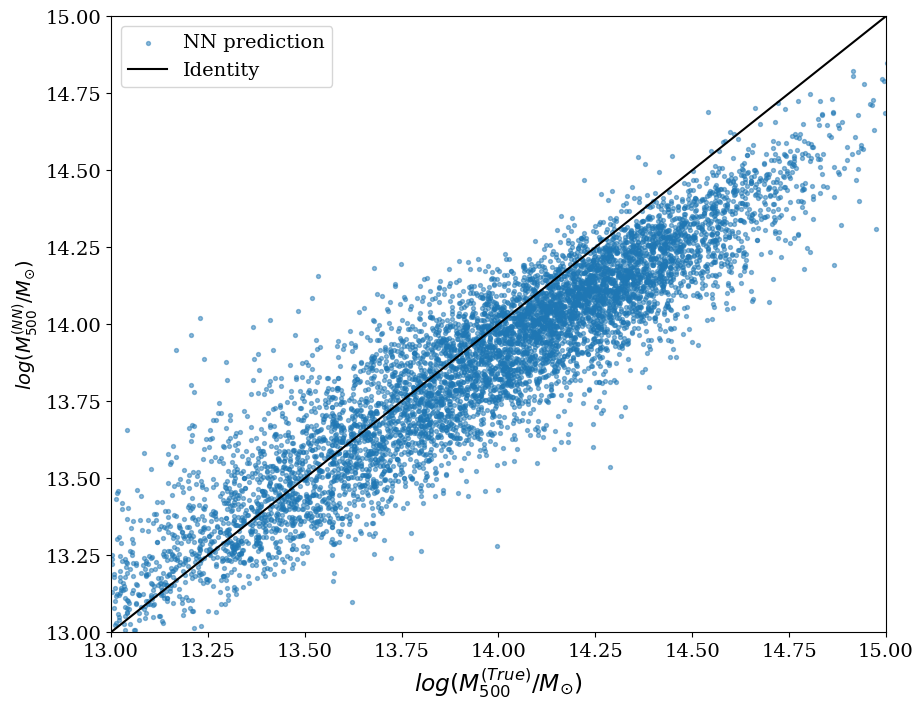
\includegraphics[width=\linewidth]{images/Chapter4/Res101V2/res101v2_training.png}
  \caption{Model predictions on the training set.}
  \label{fig:best_perf_resnet101v2_b}
\end{subfigure}
\begin{subfigure}{.46\textwidth}
  \centering
  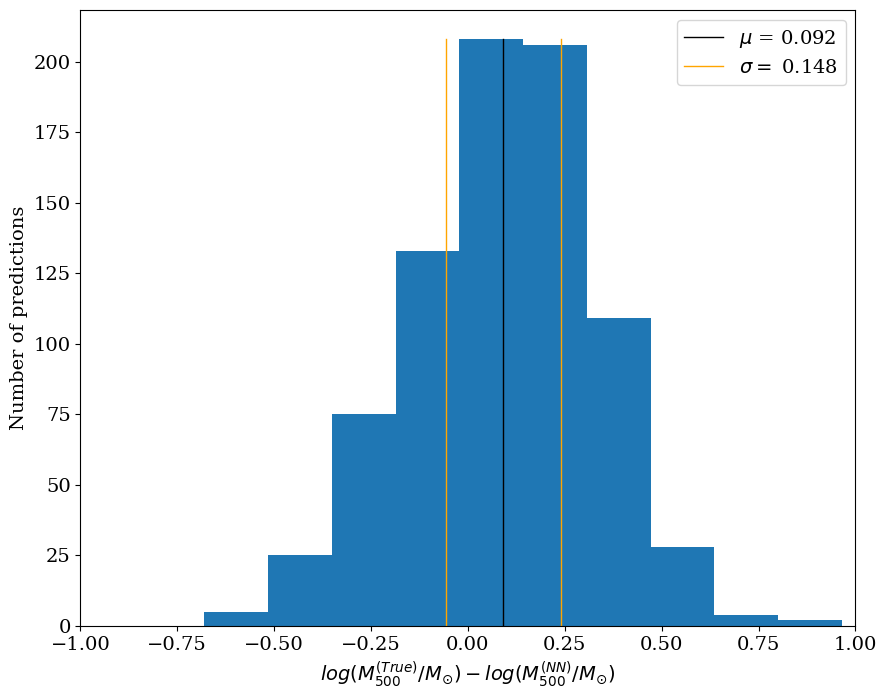
\includegraphics[width=\linewidth]{images/Chapter4/Res101V2/res101v2_test_hist.png}
  \caption{Histogram of model predictions on the test set.}
  \label{fig:best_perf_resnet101v2_c}
\end{subfigure}%
\hspace{.6em}
\begin{subfigure}{.46\textwidth}
  \centering
  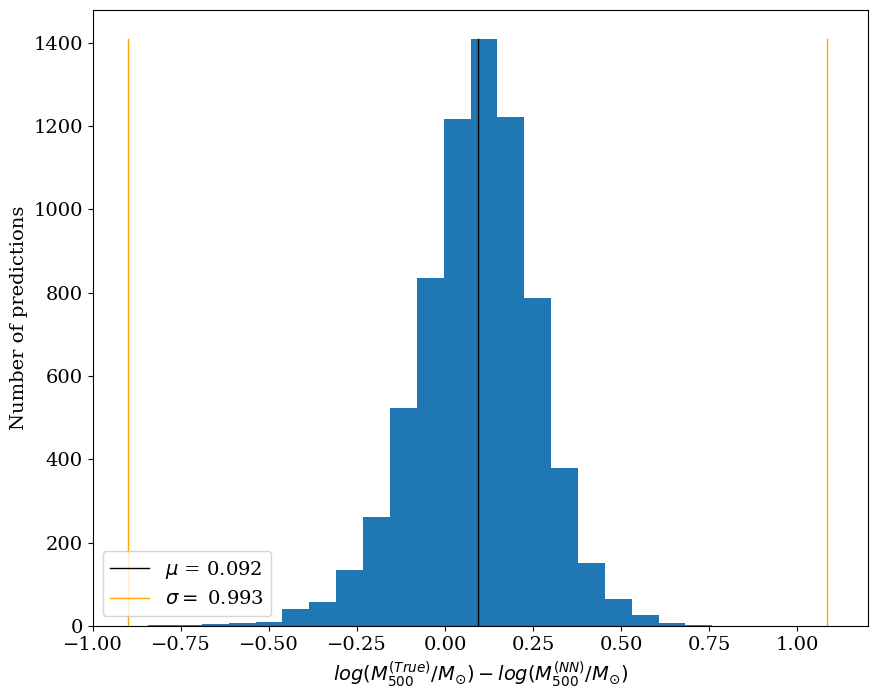
\includegraphics[width=\linewidth]{images/Chapter4/Res101V2/res101v2_training_hist.png}
  \caption{Histogram of model predictions on the training set.}
  \label{fig:best_perf_resnet101v2_d}
\end{subfigure}
\caption{Predictions on the training set had some very bad predictions, resulting in a very high $\sigma$ of $0.993$. Apart from that, the training set does not seem to be overfitted.} 
\label{fig:best_perf_resnet101v2}
\end{figure}

Interestingly, the model struggled with some of the training data by estimating a few values way too high or too low. This can be seen by the $\sigma$ of almost one. These estimations are not shown on \autoref{fig:best_perf_resnet101v2_b} and \autoref{fig:best_perf_resnet101v2_c} because they would make the important part of these plots unreadable. It is fascinating that in spite of these bad predictions, the model was still able to perform quite well.